\documentclass[11pt]{article}

\usepackage[margin=1in]{geometry}
\usepackage[utf8]{inputenc}
\usepackage[T1]{fontenc}
\usepackage{lmodern}
\usepackage{microtype}
\usepackage{graphicx}
\usepackage{booktabs}
\usepackage{hyperref}
\usepackage{xcolor}
\usepackage{listings}
\usepackage{tikz}
\usepackage{amsmath}
\usepackage{caption}
\usetikzlibrary{arrows.meta, positioning, shapes.geometric}

\hypersetup{
    colorlinks=true,
    linkcolor=blue!60!black,
    citecolor=blue!60!black,
    urlcolor=blue!60!black,
}

% ── Jac language definition for listings ──
\lstdefinelanguage{Jac}{
    morekeywords={walker, node, edge, can, has, with, entry, exit, visit,
                  report, disengage, spawn, include, import, if, elif, else,
                  for, in, while, return, not, and, or, True, False, None,
                  self, here, root, str, int, float, bool, list, dict, set},
    sensitive=true,
    morecomment=[l]{\#},
    morecomment=[s]{"""}{"""},
    morestring=[b]",
    morestring=[b]',
}

\lstset{
    language=Jac,
    basicstyle=\ttfamily\small,
    keywordstyle=\bfseries\color{blue!70!black},
    commentstyle=\itshape\color{gray},
    stringstyle=\color{red!60!black},
    numbers=left,
    numberstyle=\tiny\color{gray},
    numbersep=6pt,
    breaklines=true,
    frame=single,
    framesep=4pt,
    rulecolor=\color{black!30},
    xleftmargin=1.5em,
    aboveskip=8pt,
    belowskip=8pt,
    tabsize=4,
    showstringspaces=false,
}

\title{Implementing TPC-H on a Graph-Native Language:\\A Jac Case Study}
\author{}
\date{}

\begin{document}
\maketitle

% ════════════════════════════════════════════
\begin{abstract}
TPC-H is the industry-standard benchmark for evaluating analytical query processing,
traditionally implemented against relational database systems using SQL.
This paper presents a complete implementation of all~22 TPC-H queries
as graph walker traversals in Jac, a data-spatial programming language
in which mobile agents called \emph{walkers} carry computation to data
rather than pulling data to computation.
We map the eight TPC-H tables to typed graph nodes, foreign keys to directed
edges, and each query to one or more walker definitions that traverse the
resulting graph.
A multi-hop traversal syntax allows walkers to jump directly to target nodes
several hops away, reducing per-query code from five or more entry abilities
to one or two.
All~22 queries are verified against reference SQL answers generated at scale
factor~0.01.
\end{abstract}

% ════════════════════════════════════════════
\section{Introduction}

The TPC-H benchmark~\cite{tpch} defines a decision-support workload comprising
eight base tables and~22 analytical queries that exercise joins, aggregations,
subqueries, and sorting.
It has served as the de facto standard for comparing relational
database systems for over two decades.

Graph databases and graph-native programming languages offer a fundamentally
different computation model: data is stored as nodes and edges, and queries
are expressed as traversals rather than relational joins.
\emph{Jac}~\cite{jac} is a data-spatial programming language built on top of
Python that introduces the concept of \emph{walkers}---mobile computational
agents that move across a graph, executing abilities as they visit each node.

This paper investigates whether a graph-native language can express the full
suite of TPC-H queries.
We implement all~22 queries in Jac using multi-hop walker traversals,
verify correctness against SQL reference answers, and discuss the
patterns and trade-offs that emerge from this exercise.

% ════════════════════════════════════════════
\section{Background}

\subsection{The TPC-H Benchmark}

TPC-H models a wholesale supplier environment with eight tables:
\textsc{Region}, \textsc{Nation}, \textsc{Supplier}, \textsc{Part},
\textsc{PartSupp}, \textsc{Customer}, \textsc{Orders}, and
\textsc{LineItem}.
Foreign keys define a hierarchy of relationships.
The 22 queries range from simple single-table aggregations (Q1, Q6) to
complex multi-table joins with correlated subqueries (Q2, Q21).
A \emph{scale factor} (SF) parameter controls the dataset size;
SF\,=\,0.01 produces roughly 86{,}000 rows across all tables.

\subsection{The Jac Programming Language}

Jac extends Python with first-class graph primitives.
The key abstractions are:

\paragraph{Nodes.}
Typed graph vertices with named attributes, declared with the \lstinline|node|
keyword:
\begin{lstlisting}
node Region {
    has r_regionkey: int,
        r_name: str,
        r_comment: str;
}
\end{lstlisting}

\paragraph{Edges.}
Typed directed edges connecting nodes, declared with the \lstinline|edge|
keyword.
An edge may carry its own attributes, though in TPC-H the edges are
attribute-free labels that encode foreign-key relationships:
\begin{lstlisting}
edge region_has_nation {}
edge nation_has_customer {}
\end{lstlisting}

\paragraph{Walkers.}
Mobile computational agents that traverse the graph.
A walker has \lstinline|has| variables (persistent state carried across hops),
and \emph{abilities} that fire when the walker enters or exits a particular
node type.
Inside an ability, the \lstinline|here| keyword refers to the current node
and \lstinline|self| refers to the walker's own state.
The \lstinline|visit| statement directs the walker to move to other nodes,
and \lstinline|report| returns a result to the caller.

\paragraph{Multi-hop traversal.}
Jac supports chained edge--node filters in a single \lstinline|visit|
statement:
\begin{lstlisting}
visit [-->(?:Region)->:region_has_nation:->(?:Nation)
       ->:nation_has_customer:->(?:Customer)];
\end{lstlisting}
This causes the walker to jump directly to the \textsc{Customer} nodes,
traversing \textsc{Region} and \textsc{Nation} silently---entry abilities
fire \emph{only} on the final target nodes.

\paragraph{Graph construction.}
The operators \lstinline|++>| and \lstinline|+>: EdgeType() :+>| create
nodes and typed edges, respectively.

% ════════════════════════════════════════════
\section{Graph Schema Design}

We map each TPC-H table to a node type and each foreign-key relationship to
a directed edge type.
Figure~\ref{fig:schema} shows the resulting schema.

\begin{figure}[ht]
\centering
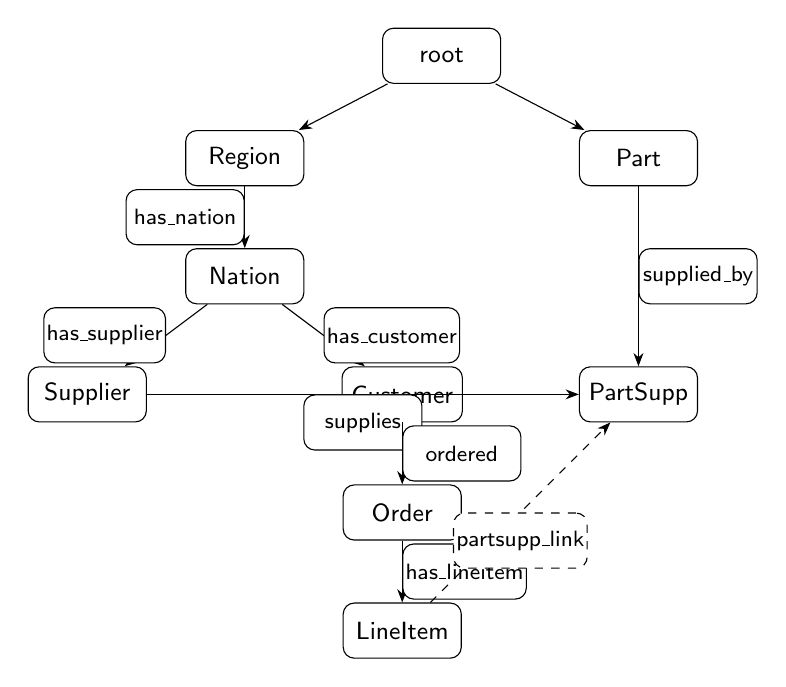
\begin{tikzpicture}[
    every node/.style={draw, rounded corners, minimum width=1.5cm,
        minimum height=0.7cm, font=\small\sffamily},
    edge_label/.style={font=\tiny\sffamily, fill=white, inner sep=1pt},
    >=Stealth,
]
    \node (root) at (0,0) {root};
    \node (region) at (-2.5,-1.3) {Region};
    \node (part) at (2.5,-1.3) {Part};
    \node (nation) at (-2.5,-2.8) {Nation};
    \node (supplier) at (-4.5,-4.3) {Supplier};
    \node (customer) at (-0.5,-4.3) {Customer};
    \node (partsupp) at (2.5,-4.3) {PartSupp};
    \node (order) at (-0.5,-5.8) {Order};
    \node (lineitem) at (-0.5,-7.3) {LineItem};

    \draw[->] (root) -- (region);
    \draw[->] (root) -- (part);
    \draw[->] (region) -- node[edge_label, left] {\footnotesize has\_nation} (nation);
    \draw[->] (nation) -- node[edge_label, left] {\footnotesize has\_supplier} (supplier);
    \draw[->] (nation) -- node[edge_label, right] {\footnotesize has\_customer} (customer);
    \draw[->] (part) -- node[edge_label, right] {\footnotesize supplied\_by} (partsupp);
    \draw[->] (supplier) -- node[edge_label, below] {\footnotesize supplies} (partsupp);
    \draw[->] (customer) -- node[edge_label, right] {\footnotesize ordered} (order);
    \draw[->] (order) -- node[edge_label, right] {\footnotesize has\_lineitem} (lineitem);
    \draw[->, dashed] (lineitem) -- node[edge_label, below] {\footnotesize partsupp\_link} (partsupp);
\end{tikzpicture}
\caption{Graph schema for TPC-H.
    Solid arrows represent the primary traversal hierarchy;
    the dashed arrow is a cross-reference from \textsc{LineItem} to \textsc{PartSupp}.
    Only \textsc{Region} and \textsc{Part} connect directly to \texttt{root}.}
\label{fig:schema}
\end{figure}

The hierarchy has two principal branches rooted at \texttt{root}:
\begin{itemize}
    \item \textsc{Region} $\to$ \textsc{Nation} $\to$
          \textsc{Customer} $\to$ \textsc{Order} $\to$ \textsc{LineItem}
          (with a fork at \textsc{Nation} $\to$ \textsc{Supplier}), and
    \item \textsc{Part} $\to$ \textsc{PartSupp}.
\end{itemize}
The \textsc{LineItem}--\textsc{PartSupp} edge acts as a cross-reference,
analogous to a composite foreign key in the relational schema.
Each \textsc{PartSupp} node also receives an incoming edge from the
relevant \textsc{Supplier} node.

% ════════════════════════════════════════════
\section{Query Implementation Patterns}

The~22 TPC-H queries, when expressed as walker traversals, fall into a small
number of recurring patterns.

\subsection{Direct Multi-Hop Aggregation}

Queries that aggregate over \textsc{LineItem} data without needing
intermediate node attributes can be expressed with a single multi-hop
\lstinline|visit| from root to lineitem.
Q1 (Pricing Summary) is the canonical example:

\begin{lstlisting}
walker Q1_PricingSummary {
    has delta: int = 90;
    has agg: dict = {};
    has cutoff: str = "";

    can on_root with Root entry {
        import datetime;
        self.cutoff = (datetime.date(1998, 12, 1)
            - datetime.timedelta(days=self.delta)).isoformat();
        visit [-->(?:Region)->:region_has_nation:->(?:Nation)
            ->:nation_has_customer:->(?:Customer)
            ->:customer_ordered:->(?:Order)
            ->:order_has_lineitem:->(?:LineItem)];
    }
    can on_lineitem with LineItem entry {
        if here.l_shipdate <= self.cutoff {
            # ... aggregate into self.agg ...
        }
    }
    can finish with Root exit {
        # ... sort and report results ...
    }
}
\end{lstlisting}

The walker starts at \texttt{root}, jumps directly to every
\textsc{LineItem} node (five hops away), and aggregates matching rows.
The \lstinline|Root exit| ability fires after all visited nodes have been
processed, serving as the finalization step.
Queries Q6, Q14, Q15, Q17, Q19, and Q20 follow this same pattern.

\subsection{Filtered Intermediate Traversal}

When a query filters on attributes of intermediate nodes, the walker must
stop at those nodes, apply the filter, and conditionally continue.
Q3 (Shipping Priority) demonstrates this pattern:

\begin{lstlisting}
walker Q3_ShippingPriority {
    has segment: str = "BUILDING",
        date: str = "1995-03-15";
    has order_map: dict = {};
    has agg: dict = {};

    can on_root with Root entry {
        visit [-->(?:Region)->:region_has_nation:->(?:Nation)
            ->:nation_has_customer:->(?:Customer)];
    }
    can on_customer with Customer entry {
        if here.c_mktsegment == self.segment {
            visit [->:customer_ordered:->(?:Order)];
        }
    }
    can on_order with Order entry {
        if here.o_orderdate < self.date {
            self.order_map[here.o_orderkey] = { ... };
            visit [->:order_has_lineitem:->(?:LineItem)];
        }
    }
    can on_lineitem with LineItem entry {
        # ... compute revenue using order_map ...
    }
}
\end{lstlisting}

The multi-hop visit from root lands the walker on \textsc{Customer} nodes.
The \lstinline|on_customer| ability checks the market segment and only
continues the traversal for matching customers.
Similarly, \lstinline|on_order| filters by date before visiting line items.
Queries Q4, Q5, Q7, Q8, Q9, Q10, Q12, Q18, and Q21 use variations of
this pattern.

\subsection{Helper Walker Pattern}

Some queries require information that spans both branches of the graph
(e.g., joining \textsc{LineItem} data with \textsc{Supplier} nation
information).
Since a walker cannot simultaneously traverse two branches, we use
\emph{helper walkers} that pre-build lookup maps:

\begin{lstlisting}
walker _BuildSuppNationMap {
    has result: dict = {};

    can on_root with Root entry {
        visit [-->(?:Region)->:region_has_nation:->(?:Nation)];
    }
    can on_nation with Nation entry {
        for supp in [->:nation_has_supplier:->](?:Supplier) {
            self.result[supp.s_suppkey] = here.n_name;
        }
    }
}
\end{lstlisting}

The main query walker spawns the helper, extracts its \lstinline|result|
map, and uses it during its own traversal:

\begin{lstlisting}
can on_root with Root entry {
    sn_helper = root spawn _BuildSuppNationMap();
    self.supp_nation = sn_helper.result;
    visit [...];
}
\end{lstlisting}

This pattern is the graph-traversal analog of a hash join in relational
processing.
Queries Q2, Q5, Q7, Q8, Q9, Q11, Q15, Q16, Q19, and Q20 use one or more
helper walkers.

\subsection{Two-Phase Traversal}

Q20 (Potential Part Promotion) requires data from the \textsc{LineItem}
subtree to determine thresholds before querying the
\textsc{Supplier}--\textsc{PartSupp} subtree.
The walker performs a first-phase traversal to collect line-item quantities,
then spawns a second-phase walker with the collected data:

\begin{lstlisting}
can finish with Root exit {
    q20_helper = root spawn _Q20Phase2(
        nation_name=self.nation_name,
        matching_partkeys=self.matching_partkeys,
        li_qtys=self.li_qtys
    );
    report q20_helper.result;
}
\end{lstlisting}

This pattern naturally arises for queries with correlated subqueries that
reference aggregates over other parts of the schema.

\subsection{LEFT JOIN Emulation}

Q13 (Customer Distribution) requires a LEFT OUTER JOIN between
\textsc{Customer} and \textsc{Orders}.
In the walker model, we initialize every customer's order count to zero
and then increment it for matching orders:

\begin{lstlisting}
can on_customer with Customer entry {
    if here.c_custkey not in self.cust_order_count {
        self.cust_order_count[here.c_custkey] = 0;
    }
    visit [->:customer_ordered:->(?:Order)];
}
can on_order with Order entry {
    # Exclude orders matching the comment pattern
    if not excluded {
        self.cust_order_count[here.o_custkey] += 1;
    }
}
\end{lstlisting}

Customers with no qualifying orders retain their zero count, preserving
the LEFT JOIN semantics.

% ════════════════════════════════════════════
\section{Data Loading and Verification}

\subsection{Data Generation}

We use the TPC-H \texttt{dbgen} tool to produce pipe-delimited
\texttt{.tbl} files at scale factor~0.01.
This yields approximately 86{,}800 nodes across all eight table types.

\subsection{Graph Construction}

A dedicated loader module (\texttt{loader.jac}) reads each \texttt{.tbl}
file, instantiates typed nodes, and connects them via typed edges using
lookup maps keyed by primary keys.
For example, each \textsc{Nation} row is connected to its parent
\textsc{Region} via a \lstinline|region_has_nation| edge:

\begin{lstlisting}
n = region_map[regionkey]
    +>: region_has_nation() :+> nation_node;
\end{lstlisting}

Loading the full SF\,=\,0.01 dataset takes approximately 4--5~minutes.

\subsection{Reference Answer Generation}

Correctness verification requires reference answers.
We load the same \texttt{.tbl} files into an in-memory SQLite database
and execute the official TPC-H SQL queries.
The results are serialized to pipe-delimited \texttt{.out} files
(one per query), which serve as ground truth.

\subsection{Verification}

After running all~22 walker queries, a verification script
(\texttt{verify\_answers.py}) compares each query's output against the
reference \texttt{.out} file, checking row counts, column values, and
sort order with tolerance for floating-point rounding.
All~22 queries pass at SF\,=\,0.01.

% ════════════════════════════════════════════
\section{Performance Observations}

While this work focuses on expressiveness rather than performance, we
note several observations at SF\,=\,0.01.

The~22 queries fall into three runtime tiers:
\emph{fast} queries (Q2, Q7, Q8, Q11, Q16, Q17, Q22) complete in
0.3--3\,seconds;
\emph{medium} queries (Q3, Q5, Q10, Q13) require 1--6\,seconds;
and \emph{lineitem-traversal} queries (Q1, Q4, Q6, Q9, Q12, Q14, Q15)
take approximately 12\,seconds each, as they visit all $\sim$60{,}000
line-item nodes.

The Jac walker runtime is implemented on top of Python and uses
recursive function calls for graph traversal.
At SF\,=\,0.01, the traversal depth can exceed Python's default recursion
limit, requiring it to be raised to 500{,}000 or higher.
This limits scalability to larger scale factors without runtime
modifications.

The multi-hop traversal syntax provides a significant speedup over the
single-hop alternative.
In the single-hop version, separate entry abilities fire at every
intermediate node type, incurring Python function-call overhead at each
of the $\sim$86{,}000 nodes.
Multi-hop traversal skips intermediate abilities entirely, visiting only
the target nodes.

% ════════════════════════════════════════════
\section{Discussion}

\paragraph{Traversal vs.\ Joins.}
Graph traversal is a fundamentally different computation model from
relational joins.
In SQL, a five-table join is a single declarative statement that the
optimizer can reorder.
In Jac, the same operation is an explicit path through the graph, with
the programmer controlling traversal order.
This gives more control but shifts optimization responsibility to the
developer.

\paragraph{Walker State as Hash Tables.}
Many TPC-H queries require combining data from multiple tables.
In the walker model, this is achieved by accumulating data into
\lstinline|has| variables (typically dictionaries) as the walker
traverses intermediate nodes, then using that state at deeper levels.
This is functionally equivalent to building hash tables for hash-join
execution in relational engines.

\paragraph{The Helper Walker Pattern as Subquery Execution.}
Spawning helper walkers to build lookup maps before the main traversal
mirrors how relational engines execute correlated subqueries by
materializing intermediate results.
Jac makes this explicit: the programmer decides what to pre-compute
and what to compute inline.

\paragraph{Limitations.}
The current implementation has several limitations:
(1)~Every query traverses from \texttt{root}, as the language restricts
traversal origins to \lstinline|here| (the current node) rather than
arbitrary variable references;
(2)~there are no secondary indexes, so selective queries must still visit
all nodes along the path;
(3)~Python's recursion limit constrains the graph size; and
(4)~the persistent graph database accumulates data across runs and must
be manually cleared.

% ════════════════════════════════════════════
\section{Conclusion}

We have demonstrated that all~22 TPC-H queries can be faithfully
expressed as graph walker traversals in Jac, a data-spatial programming
language.
The multi-hop traversal syntax reduces per-query implementation
complexity from five or more entry abilities to one or two, while
maintaining correctness against SQL reference answers.

Five recurring patterns---direct multi-hop aggregation, filtered
intermediate traversal, helper walkers, two-phase traversal, and
LEFT~JOIN emulation---cover the full range of TPC-H query types.
These patterns suggest that graph-native languages can serve as a
viable alternative paradigm for expressing analytical workloads,
though performance optimization and scalability remain open challenges.

Future work includes testing at larger scale factors, comparing
performance with established graph databases, and exploring language-level
optimizations such as parallel walker execution and automatic index
generation.

% ════════════════════════════════════════════
\begin{thebibliography}{9}

\bibitem{tpch}
Transaction Processing Performance Council,
``TPC-H Benchmark Specification,''
Revision~3.0.1, 2022.
\url{https://www.tpc.org/tpch/}

\bibitem{jac}
J.~Jaseci,
``Jac Language Documentation,''
2024.
\url{https://www.jac-lang.org/}

\bibitem{jaseci}
Y.~Mars \emph{et al.},
``Jaseci: A Data-Spatial Programming Framework,''
2023.
\url{https://github.com/Jaseci-Labs/jaseci}

\end{thebibliography}

\end{document}
